% Theoretical background
 %if the chapter heading starts close to bottom of the page, force a line break and remove the vertical vspace
\vspace{21.5pt}
\chapter{Fuzzy Testing}
In this chapter, the focus shifts to fuzz testing as a specialized technique within the realm of
software testing. The chapter starts with an introduction to Fuzzy testing.  The next section describes
about the history and evolution of fuzz testing, providing a solid foundation for understanding the
development of this technique over time. The next section delves into the reasons behind the
utilization of fuzz testing, the process of how it is performed, and the aspects of software
that can be targeted for fuzzing. Following that, the working process and components of
fuzzing are explored, offering a detailed explanation of the various elements involved in fuzz testing,
such as the Fuzzers, the test harness, and the monitoring tools. Finally, the last section of this chapter
concludes with success of fuzzy testing including embedded projects.

\section{Fuzzing: An Introduction}

Fuzzy testing, also known as ``fuzzing,'' has emerged as a prominent vulnerability discovery
technique in software testing. This approach involves iteratively and randomly generating automatic
inputs to test a target program, with the aim of identifying software bugs. As the
System Under Test (SUT) is monitored, fuzzing tools, or ``Fuzzers'', continuously generate
significant amounts of valid and invalid data, which are then inserted into the target application.
The Fuzzers then observe and report any crashes that occur during the testing
process\cite{klees2018evaluating}\cite{li2018fuzzing}.

Fuzzy testing has gained popularity due to its ability to discover previously unknown
vulnerabilities in software, which may be missed by traditional testing methods.
Additionally, fuzzing can be used to test software across multiple platforms and
configurations, which is especially useful for complex applications.
The random and iterative nature of fuzzing makes it a powerful tool for testing software that
has complex, non-linear behavior\cite{klees2018evaluating}.

It is important to note that while fuzzy testing has become a widely accepted approach to
vulnerability discovery, it is not a substitute for other testing methods.
Instead, it is often used in conjunction with other techniques to provide a comprehensive
approach to software testing. The use of fuzzing has become increasingly important as software
systems become more complex and diverse, making it an essential technique for ensuring the security
and reliability of modern software system\cite{kim2011efficient}.

Fuzzy testing, a systematic method for detecting software vulnerabilities,
comprises several distinct stages. First, researchers must identify the target application,
which could range from the entire application to a specific file or library within it\cite{segedyfuzz}.
Next, the input data transmitted from the client to the target must be determined.

In the third stage, test case generation occurs, involving the creation of various combinations of
valid and malformed data in formats such as binary or files. The fourth stage involves fuzzers
executing the target program using the inputs generated in the previous stage, and then
halting the execution after a pre-defined timeout period. During this stage, fuzzers
record any crashes or unexpected behavior that may arise.

The fifth stage, known as the analysis phase, requires fuzzers to examine or monitor the results
obtained in the previous stage. Lastly, the sixth stage entails determining whether any observed
crashes or unexpected behavior during the target program's execution indicate potential
vulnerabilities. This analysis process involves verifying if the anomalous behavior is
attributable to a legitimate security issue or merely a benign error.
\clearpage
The figure:\ref{fig:fuzzy_testing_phases} describes different stages of fuzzing.

\begin{figure}[h!]
        \centering
        \AltText{Fuzzing Stages}{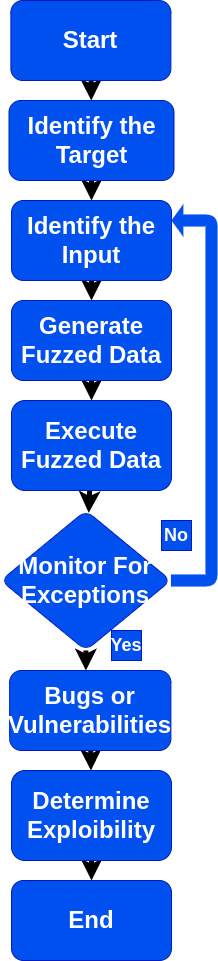
\includegraphics[width=6.1cm]{fuzzy_testing_phases}}
        \caption{Fuzzing Stages\cite{segedyfuzz}\cite{9742291}.}\label{fig:fuzzy_testing_phases}
\end{figure}

Overall, the use of fuzzy testing provides a valuable approach to identifying potential
vulnerabilities in software systems. By generating many test cases with both
valid and malformed data, fuzzing techniques can expose weaknesses in software that may not be
detected through traditional testing methods. Additionally, the analysis of the results of the
fuzzing process enables software developers to identify and address potential security issues
before they can be exploited by malicious actors.\newline

\subsection{History and Evolution of Fuzzy Testing}
Although, a relatively new automation technique, the term `fuzzing' or `fuzz testing'
is first established by Barton Miller in the year 1988\cite{takanen2009fuzzing} as class project.
However, originally fuzzing meant as ad-hoc testing or random testing in some mission-critical
applications. The first open-source fuzz testing framework came out during the year
2007\cite{takanen2009fuzzing}.

Despite being a relatively new automation technique, the term ``fuzzing'' or  ``fuzz testing''
was first introduced in 1988 by Barton Miller as part of a class project\cite{takanen2009fuzzing}.
Originally, fuzzing referred to ad-hoc or random testing methods employed in certain mission-critical
applications. However, over time the term has evolved to refer specifically to the automated
generation and testing of large numbers of input values for software systems.

Notably, the first open-source fuzz testing framework was released in 2007\cite{takanen2009fuzzing}.
This framework marked a significant milestone in the evolution of fuzzing as a formalized technique
for software testing, and has since been followed by numerous other frameworks and tools that
support fuzz testing across a wide range of software systems.

The development of fuzzing as a specialized technique for software testing has enabled
researchers and practitioners to more effectively identify and address potential vulnerabilities
in software systems. As the technology and tools for fuzzing continue to evolve, it is likely that
the use of this technique will become even more widespread in the future, helping to ensure the
security and reliability of software systems in a wide range of applications.


Over time, the term fuzzing has evolved to become a critical technique for hackers,
cybersecurity personnel, software developers, and testers. In its early stages,
fuzzing was primarily used to uncover memory corruption bugs, but its capabilities
have since expanded significantly.

Modern fuzzing frameworks are now more flexible and customizable, allowing them
to be applied to any layer of software. This has made fuzzing an increasingly
popular and effective technique for identifying and addressing potential
vulnerabilities in software systems. As a result, fuzzing has become an
important tool for ensuring the security and reliability of software systems
in a wide range of applications.\newline

\subsection{Why, How and What to Fuzz}

Fuzz testing is a valuable technique for assessing the security, correctness,
and stability of software systems. Specifically, it is particularly useful for
software systems that receive inputs from untrusted sources. In such cases,
fuzz testing can help to confirm the reliability of the inputs and ensure that
they can be trusted.

Moreover, fuzz testing can also be used to verify the correctness of complex
software programs, and to ensure that they operate as expected. This is
particularly important for software that is critical to the functioning of a
larger system or application.

Finally, even in cases where the inputs to a software system are trusted,
fuzz testing can be valuable for establishing the stability of the program.
By subjecting the system to high volumes of inputs, fuzz testing can help to
identify any performance or stability issues that may arise under stress or heavy usage.

In summary, fuzz testing is a versatile and important technique for assessing
the security, correctness, and stability of software systems across a wide
range of applications and use cases.

Fuzzing is a useful technique for discovering programming issues,
errors, and vulnerabilities in software systems that may not be
specifically related to their requirements or intended functionalities.
However, it should not be seen as a substitute for other types of testing,
such as functional, unit, integration, and system testing.

In particular, fuzz testing is often used to identify issues such as memory leaks,
address corruptions, and buffer overflows on embedded devices, and can be
performed with or without access to the source code.

To achieve the best results, fuzz testing should be performed continuously.
By continually subjecting software systems to randomized inputs, fuzz testing
can help to identify issues that may arise over time or in response to changing
conditions. As such, fuzz testing should be seen as an important supplement to
other types of testing, helping to ensure the overall security, reliability,
and performance of software systems.

After deciding to perform a fuzzing test on an application, it is critical
to identify the specific targets for the test, including what and how to fuzz.
Applications that are exposed to and accept inputs from untrusted users are
prime candidates for fuzz testing. However, in large and complex applications,
it can be challenging to identify the specific code paths that are exposed to
untrusted inputs.

To address this challenge, it is important to find and define entry points that
can be used by the fuzzers to mimic untrusted inputs. Common entry points for
fuzz testing include file inputs, network inputs, and command line inputs.
By identifying and defining these entry points, fuzz testers can focus their
efforts on the areas of the application that are most likely to be vulnerable
to attacks or other forms of misuse.

Overall, selecting the right targets for fuzz testing is critical to the
success of the test, and requires careful analysis and planning to ensure
that the most vulnerable areas of the application are thoroughly tested.

Below given examples applications targets where fuzzing has been successful.\label{par:target_categories}

\begin{itemize}
        \item Databases: Oracle, SQL
        \item Text editors: vim, OpenOffice
        \item Processors
        \item Linux OS kernels, drivers
        \item Parsers: xml, pdf
        \item Crypto libraries: OpenSSL, LibreSSL, EverCrypt
        \item Browsers: Chrome, Firefox
        \item Network protocols, libraries
        \item Media Codecs: Audio, Video\newline
\end{itemize}


\subsection{Working Process and Components of Fuzzing}

A traditional fuzzing test case consists of four stages: test case generation,
execution, monitoring, and analysis. The test begins with the generation of many
inputs that are designed to break the program. These inputs can take
various forms, such as different file formats, binary executables, or network
commands. However, generating broken inputs that can cause the program to fail
is a challenging task.


To address this challenge, two common generators are used to generate inputs for
fuzzers: \textit{mutation-based generators} and \textit{generation-based generators}.
Mutation-based generators mutate the existing input data, also known as test \gls{corpus},
to create new test data, while generation-based generators create entirely
new inputs for the fuzzers\cite{li2018fuzzing}.


After generating the inputs in the first stage, the test cases are fed to
the program, and the fuzzing process continues until the program crashes or hangs.
During execution, fuzzers monitor the crashes and exceptions using tools
like sanitizers, which can detect specific system signals, crashes, and other violations.

In the analysis stage, the focus is on finding the root cause of the issues
identified during monitoring. This stage is critical for understanding the nature and
severity of the bugs, errors, or vulnerabilities discovered through fuzzing.
By identifying the root cause of these issues, developers and testers can take
steps to fix them and improve the overall quality and security of the software.

In summary, the traditional fuzzing test case involves a structured approach
to generating and executing test cases, monitoring program behavior,
and analyzing the results. By following this process, testers can uncover hidden
bugs and vulnerabilities, allowing developers to fix them before they can be
exploited by attackers.

The figure:\ref{fig:general_process_fuzzing} describes different general process of fuzzing, and
its dependencies.

\begin{figure}[h!]
        \centering
        \AltText{General Process Fuzzing}{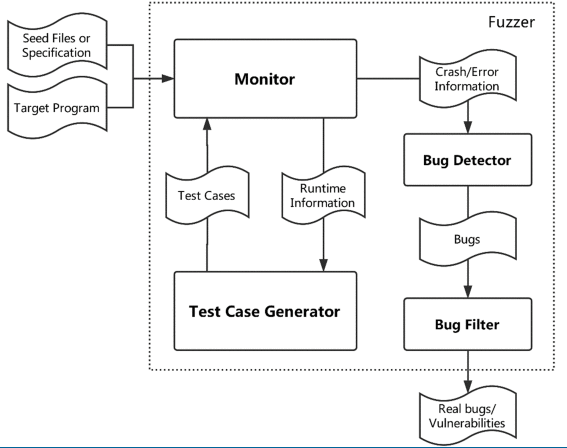
\includegraphics[width=12.1cm]{general_process_fuzzing}}
        \caption{General Process Fuzzing\cite{liang2018fuzzing}.}\label{fig:general_process_fuzzing}
\end{figure}

\textbf{Target:} The target of a fuzzing test is the \acrlong{sut}, which is
typically a binary program that the fuzzers aim to target.

\textbf{Monitor:} The monitor component collects execution information about the target,
such as code coverage and data flow. Gray and white box fuzzers
incorporate the monitor component as part of their design.

\textbf{Test case generator:} In order to generate inputs for the fuzzing process,
fuzzers utilize either mutation or generation based methods. Mutation-based
generators randomly mutate valid inputs or use predefined strategies for
generating inputs during runtime. On the other hand, generation-based methods
create new seeds from the specification. Typically, the inputs used in fuzz
testing are a mixture of valid and invalid inputs that pass initial validation
but may still trigger bugs.

\textbf{Bug Detector:} The bug detector is a key component in fuzzers that is designed
and implemented to identify potential bugs in the target program.
During the fuzzing process, the bug detector collects and analyzes the stack
traces from the crashes and errors that occur as a result of the test inputs.
Some fuzzers also use debuggers as an alternative to the bug detector for
identifying bugs in the target program

\textbf{Bug Filter:} It is important to filter out non-security related bugs
from the overall reported bugs. However, this filtering process can be a manual and
time-consuming task. As a result, ongoing research is being conducted to develop
methods to automate and improve this process.

\textbf{Sanitizers}
There are many ways an unforced error can get introduced to a computer program. These problems are not
easy to detect by the naked eyes and mostly about memory leaks, threading related issues. Sanitizers, a set
of dynamic testing tool which help to detect these issues during the runtime. Used by the
compilers such as \textit{gcc} and \textit{clang} to buffer overflows, uninitialized memory violations
and threading problems.

\section{Classification of Fuzzing Methods}\label{sec:fuzzing_methods}
Fuzzing tools and methods are classified into three main categories: gray-box, white-box and
black-box fuzzing.

\subsection{White-Box Fuzzing Method}

White-box fuzzing is a systematic technique for enumerating different interesting paths in a
program by using program analysis and constraint solvers. It relies on the internal logic
of the target program and is based on the technique called \textit{symbolic execution}\cite{cadar2013symbolic}.
This method was proposed to overcome the limitations of black-box fuzzing and was first
\Citeauthor{godefroid2008automated}. To scan through the target program, white-box fuzzing uses
a search technique called coverage-maximizing heuristic search
algorithm\cite{godefroid2008automated}\cite{liang2018fuzzing}.

Before starting the fuzzing process, white-box fuzzing requires the necessary information
from the target program to generate the inputs. It collects all the conditional paths of the target
program by applying \acrlong{smt} formulas. For example, it uses the formula
\begin{math}i[0] = 42 \land i[0] - i[1] > 7\end{math}, where \textit{i} is the set of inputs
that traverse the target\cite{bohme2021fuzzing}. The path condition is then calculated and mutated
and sent to a constraint solver to generate new paths and skip the blocks.
The main goal of white-box fuzzers is to reach the maximum execution paths and requirements.


One of the advantages of white-box fuzzing is that it can cover maximum coverage by generating
better and more interesting test cases. However, numerous execution paths can lead to stability and
compatibility issues in real-world software\cite{lomeli2022security}\cite{liang2018fuzzing}.
Some existing white-box fuzzers are SAGE\cite{godefroid2012sage}, KLEE\cite{cadar2008klee},
BitFuzz\cite{caballero2010input}.\newline

\subsection{Black-Box Fuzzing Method}
Black-box testing method involves generating inputs to test the target program without any
internal knowledge or specifications. The fuzzing process begins by randomly mutating
the valid inputs or generating new inputs. Examples of mutation data include flipping random bits
and bytes in a seed file, byte copies, and removal\cite{jaaskela2016genetic}.
Generational-based approaches utilize grammar and input-specification knowledge\cite{kim2013automatic}.

The fuzzing process ends after a predefined time has been exhausted. Popular black-box fuzzers
include Peach\cite{PeachFuz35:online}, Trinity\cite{GitHubke76:online} and
Funfuzz\cite{GitHubMo73:online}.\newline

\subsection{Gray-Box Fuzzing Method}
The combination of black-box and white-box fuzzing utilizes \textit{code instrumentation}
to provide feedback and obtain code coverage of the target program during runtime\cite{bohme2021fuzzing}.
This approach employs genetic algorithm mutation strategies to generate new inputs which serve as
new control locations to cover additional coverage paths. Feedback received from the coverage
enables the fuzzers to reach more coverage, including tracing the taint data flow, in a method known
as gray-box \textit{taint-analysis}\cite{bekrar2012taint}.

To detect bugs and vulnerabilities, assertions are injected by sanitizers into the target program.
Unlike the white-box method, the gray-box method utilizes runtime information to generate test cases.
Some well-known gray-box fuzzers include AFL++\cite{257204}: a fork
of \gls{afl}\cite{GitHubgo92:online}, LibFuzzer\cite{libFuzze17:online} and Honggfuzz\cite{GitHubgo89:online}.\newline

\subsection{Choose a Fuzzing Method}
In software testing, a `bug' refers to a defect in the software logic that causes unexpected or
incorrect output. The primary objective of fuzz testing is to identify and eliminate such bugs
in a system. In order to achieve this objective, selecting an appropriate fuzzing target is of
utmost importance. While black-box fuzzers are simple and lightweight, they may not be capable
of achieving high levels of code coverage and are more effective in uncovering `shallow`
bugs. On the other hand, white-box and gray-box fuzzers are adept at detecting  `hidden' bugs
that are difficult to identify. Although the implementation of these fuzzers is more complex
and time-consuming, they offer comprehensive and in-depth testing capabilities.

When considering fuzz testing methods, two important factors to consider are precision and efficiency,
as well as the quality of the results. A `dumb' fuzzer simply mutates a valid input by
randomly changing some bytes, while a `smart' fuzzer generates inputs from scratch.
The black-box fuzzing approach is known for its precision and efficiency, while the white/gray
box methods tend to produce higher quality results. Careful consideration of these factors is
essential when selecting an appropriate fuzz testing method for a given software system.

The two factors are:
\begin{enumerate}
        \item Time and Budget
        \item Input format of the target program e.g, network protocol, compiler
\end{enumerate}

\section{Implementing the Art of Fuzzing}
As per the section \hyperref[sec:fuzzing_methods]{Classification of Fuzzing Methods} below questions
should be considered when building and implementing fuzzing with fuzzers.

\begin{itemize}
        \item How to do seed selection and generation.
        \item What makes a good \gls{fuzz_target} and how to validate the inputs.
        \item What to consider with the test cases which indicates crashes.
        \item How to make good use of information during the runtime.
        \item How can we achieve scalability improvements.\newline
\end{itemize}

\subsection{Generation and Selection of Seed}

In the context of fuzz testing, a \textit{seed corpus} refers to a set of files that are representative of
the inputs that the target program can accept. The quality of the seed corpus can significantly
impact the results of the fuzzing process. Therefore, it is crucial to generate or select a
seed corpus that can help achieve 100\% coverage.

When selecting a seed corpus, it is advisable to avoid using larger files if the same level of
coverage can be achieved with smaller ones. However, as storage is typically cheap, it may be
possible to compress larger seed files to reduce their size.

Another approach to improving code coverage, proposed by \Citeauthor{kim2011efficient}\cite{kim2011efficient},
involves analyzing the fields of binary files during the fuzzing process. This approach involves
tracking and analyzing stack frames, assembly codes, and registers to identify potential new inputs
that can improve coverage.\newline

\subsection{A Good Fuzz Target and Validation of Inputs}
In the context of fuzz testing, the term `fuzz target' refers to the item being tested.
This item can take many forms, such as a command line tool or a hardware device, and is
characterized by its ability to accept inputs and provide results. The effectiveness of
the fuzz testing process depends on the quality of the fuzz target and its ability to
accurately represent the behavior of the real-world system or application being tested\cite{238602}.

\subsubsection{A Good Fuzz Target}
Below given is an example of a fuzz target written in C with \textit{LLVM libFuzzer}\cite{libFuzze17:online},
\begin{lstlisting}[language=C]
extern "C" int LLVMFuzzerTestOneInput (const uint8_t  *Data,
size_t Size) {
        DoSomethingInterestingWithMyAPI(Data, Size);
        return 0;  // Values other than 0
        // and -1 are reserved for future use.
}
\end{lstlisting}

The function \textit{LLVMFuzzerTestOneInput} of the fuzzer \textit{LLVM libFuzzer} takes two arguments,
the address of the data to store and size. The API of the fuzz target is called in the next steps of
fuzzing.

It is crucial to keep the following aspects in mind when creating a fuzz target\cite{libFuzze17:online}:

\begin{itemize}
        \item The \gls{fuzzing_engine} must execute the fuzz target multiple times within the same process.
        \item The fuzz target must accept inputs ranging from valid to invalid, including empty and malformed inputs.
        \item When the fuzz target stops or exits, it signals the presence of a bug in the system.
        \item The execution of the fuzz target should be fast, with minimal logging and memory consumption.
        \item Any global state that the fuzz target relies on must not be modified. For example,
        calling\begin{math} \textit{malloc()}\end{math} can modify global state.
        \item The fuzz target should be integrated into \textit{continuous integration}.
        \item The fuzz target must be deterministic, meaning it should not rely on randomness.
        \item A good fuzz target should be fast, as multiple iterations are required in the search algorithm.
        \item Memory consumption should be low to avoid out-of-memory errors.
        \item A good fuzz target must avoid timeouts and out-of-memory errors.
\end{itemize}

\subsubsection{Input Validations}
Fuzzing offers the main advantage of generating test cases quickly. However, when the fuzz target
being tested has input validations, the generated test cases may not be useful. Hence, it is
crucial to exercise caution when creating test cases in such scenarios.

\textbf{Integrity Validation:}
Integrity validation is a crucial aspect of maintaining data integrity in various inputs
such as file formats and network protocols. To ensure the integrity of the data,
checksum mechanisms are used, which provide validation at both the sending and receiving ends.
In this regard, a fuzzer named \textit{TaintScope}, developed by \citeauthor{wang2010taintscope},
is used to mutate the hot bytes in the input, which helps in generating new test cases. However, to pass the
integrity validation, the checksum is reverted to its original state. This approach enables
the detection of vulnerabilities that might arise in the process of transmitting data,
which could compromise the integrity of the system\cite{wang2010taintscope}.

\textbf{Format Validation:}
Fuzz targets such as Android devices, compilers, and interpreters have format requirements that
must be met by inputs in order to be accepted for testing. However, in cases where inputs
do not conform to these formats, they are rejected by the system. To avoid format-based validation,
a \textit{Grammar}-based solution can be employed. For instance, \Citeauthor{cao2015towards},
developed a scanner for fuzz targets on Android devices, which is capable of evading the
initial format validation and allowing the fuzz testing process to continue without
interruption\cite{cao2015towards}.

\textbf{Environment Validation:}
Environment validation is a crucial aspect of testing, which checks the validity of configurations,
runtime status, and other environmental factors. Fuzzing tools, such as FuzzDroid\cite{rasthofer2017making},
utilize a combination of static and dynamic analysis to generate an Android runtime environment.
The tool employs a search-based algorithm to identify potential vulnerabilities, which helps in
enhancing the overall security of the system. Through this approach, FuzzDroid can effectively
identify and address issues related to syntactic and semantic validity, ultimately improving the
reliability and performance of the system.


\textbf{Input Coverage:}
Achieving high input coverage is critical to uncovering vulnerabilities in a target system.
Various techniques have been proposed to improve the input coverage of a fuzzer.
One such tool is the \textit{semi-valid coverage (SVCov)} tool, proposed by  \Citeauthor{tsankov2013semi},
SVCov helps increase the existing input coverage by generating inputs that are close to
valid inputs but still contain errors or faults that can trigger bugs in the system under test\cite{tsankov2013semi}.

Another technique to enhance input coverage is through the use of specialized fuzzers such as \textit{Artfuzz},
which was proposed by \Citeauthor{chen2016dynamically}. Artfuzz is designed to find non-crash buffer overflow
vulnerabilities by identifying inputs that can trigger buffer overflows but do not cause the system to crash.
By uncovering such vulnerabilities, Artfuzz helps improve the security of the target system\cite{chen2016dynamically}.

\subsubsection{Isolating Crashes and Test Cases}
Fuzzing often causes crashes in the target systems. These crashes can be huge in numbers and often
takes a large amount of time for analyzing. Due to time and budget often the most priority bugs get
fixed by the developers. Therefore, it is really important for the testers to isolate or filter
the test inducing crashes and take the most useful test cases into account.

\Citeauthor{chen2013taming} introduced a ranking based to isolate the crashes and test cases\cite{chen2013taming}.
In this method, the test cases which can cause bugs, and they are different in nature are ranked accordingly.
There are other methods for isolating the crashes such as clustering methods, differentiating the crashes based
on their uniqueness and debug information. The stack traces play an important role in determining the uniqueness
of the test cases and therefore need to recorded while doing the fuzzing. Another simpler way to determine the
uniqueness is to trace the execution path. Fuzzers like AFL\cite{GitHubgo92:online} determines a crash is unique
when it does not find the execution path. The uniqueness helps in isolating the crashes, the outputs and saves
time when analyzing them. Trimming of the test cases is another method of isolating the crashes and test cases.
A large size test case can take more time to execute and then more time for analysis. In mutation based fuzzers,
in which the test cases are developed and mutated during the run time usually fall into this category. Hence, trimming
of the test cases is needed from time to time while fuzzing and which can improve the overall efficiency. Trimming
is usually done by removing the identical data-blocks which can not influenced the execution path anymore
by comparing them with the original one.

\subsubsection{Runtime Information During Fuzzing}
To get code coverage and data flow which are runtime information,  symbolic execution and dynamic
analysis techniques are used. Although these techniques help in finding the `hidden' bugs, these smart
fuzzing techniques are low in efficiency.


Path Explosion is one of the biggest problem in symbolic execution during fuzzing run time. A conditional branch
in any target program can have a numerous execution paths and this can lead to Path Explosion.
\Citeauthor{godefroid2007compositional} proposed to have \textit{function summaries} in low level
functions. This can lead to less number of execution paths as the higher level functions can
reuse them\cite{godefroid2007compositional}. Heuristic search algorithms such as random path selection
and automatic partial loop summarization help to find the most relevant paths\cite{liang2018fuzzing}.

Complex programs can cause imprecision symbolic execution. Methods such as CUTE\cite{sen2005cute} helps
in making the symbolic execution more cost effective.

During the runtime, \textit{Undertainting} is another problem where without any direct assignment The
variable is transferred. \Citeauthor{kang2011dta++} has proposed that to Undertainting, it is essential to
neglect the input data flow if the input is tainted\cite{kang2011dta++}.

\section{Successes Of Fuzzing}
Fuzzy testing has been extremely effective technique since its inception in the late 1980s in discovering
long-standing bugs, vulnerabilities and improving the quality and security of software. Over the years,
wide range of applications shown in paragraph\ref{par:target_categories}, have been successfully fuzzed
and critical security vulnerabilities have been found that could have been exploited by malicious actors.
\clearpage
The table:\ref{tab:vulnerabilities_examples} showcases examples of vulnerabilities discovered by
fuzzing tools and affected components.

% \begin{longtable}{|p{2cm}|p{3cm}|p{8cm}|}
% \caption{Examples of Vulnerabilities Discovered by Fuzzing Tools}
% \label{tab:vulnerabilities_examples}\\
% \hline
% \textbf{Fuzzing Tool} & \textbf{CVE ID} & \textbf{Description and Affected Component} \\
% \hline
% \endfirsthead
% \multicolumn{3}{c}{\tablename\ \thetable\ -- \textit{Continued from previous page}} \\
% \hline
% \textbf{Fuzzing Tool} & \textbf{CVE ID} & \textbf{Description and Affected Component} \\
% \hline
% \endhead
% \hline \multicolumn{3}{r}{\textit{Continued on next page}} \\
% \endfoot
% \hline
% \endlastfoot
% AFL & CVE-2014-0160 & Heartbleed vulnerability in OpenSSL, affecting the TLS heartbeat extension\cite{durumeric2014matter} \\
% \hline
% AFL & CVE-2014-6271 & Shellshock vulnerability in the Bash shell, allowing remote code execution\cite{shetty2018shellshock} \\
% \hline
% libFuzzer & CVE-2016-1839  & Heap buffer overflow in ImageIO, affecting image decoding in macOS and iOS \\
% \hline
% syzkaller & CVE-2017-2636  & Double fetch vulnerability in the Linux kernel, allowing privilege escalation\cite{wang2017double} \\
% \hline
% go-fuzz & CVE-2016-3959  & Denial of service vulnerability in Go's standard library, affecting the HTTP/2 implementation \\
% \hline
% Honggfuzz & CVE-2017-15650  & Heap buffer overflow in Poppler, affecting PDF rendering\cite{haller2013dowsing} \\
% \hline
% % Facebook's Sapienz & N/A & Automated testing of Android apps, leading to crash fixes and improvements \\
% % \hline
% \end{longtable}

\begin{table}[h!]
\centering
\begin{tabularx}{\textwidth}{@{}>{\raggedright\arraybackslash}p{2cm}>{\raggedright\arraybackslash}p{3cm}X@{}}
\toprule
\textbf{Fuzzing Tool} & \textbf{CVE ID} & \textbf{Description and Affected Component} \\
\midrule
AFL & CVE-2014-0160 & Heartbleed vulnerability in OpenSSL, affecting the TLS heartbeat extension\cite{durumeric2014matter} \\
\addlinespace
AFL & CVE-2014-6271 & Shellshock vulnerability in the Bash shell, allowing remote code execution\cite{shetty2018shellshock} \\
\addlinespace
libFuzzer & CVE-2016-1839  & Heap buffer overflow in ImageIO, affecting image decoding in macOS and iOS \\
\addlinespace
syzkaller & CVE-2017-2636  & Double fetch vulnerability in the Linux kernel, allowing privilege escalation\cite{wang2017double} \\
\addlinespace
go-fuzz & CVE-2016-3959  & Denial of service vulnerability in Go's standard library, affecting the HTTP/2 implementation \\
\addlinespace
Honggfuzz & CVE-2017-15650  & Heap buffer overflow in Poppler, affecting PDF rendering\cite{haller2013dowsing} \\
\bottomrule
\end{tabularx}
\caption{Examples of Vulnerabilities Discovered by Fuzzing Tools}
\label{tab:vulnerabilities_examples}
\end{table}

% \clearpage
The table:\ref{tab:bugs_found_overview} provides a broader overview of the number of bugs found by
different fuzzing tools in various projects.

% \begin{longtable}{|p{1cm}|p{2cm}|p{3cm}|p{7cm}|}
% \caption{Overview of Bugs Found by Fuzzing Tools in Various Projects}
% \label{tab:bugs_found_overview}\\
% \hline
% \textbf{Year} & \textbf{Organization/Researchers} & \textbf{Fuzzing Tool/Project} & \textbf{Achievements} \\
% \hline
% \endfirsthead
% \multicolumn{4}{c}{\tablename\ \thetable\ -- \textit{Continued from previous page}} \\
% \hline
% \textbf{Year} & \textbf{Organization/Researchers} & \textbf{Fuzzing Tool/Project} & \textbf{Achievements} \\
% \hline
% \endhead
% \hline \multicolumn{4}{r}{\textit{Continued on next page}} \\
% \endfoot
% \hline
% \endlastfoot
% 1999 & OUSPG & PROTOS & Found security vulnerabilities in Voice over IP (VoIP) implementations\cite{roning1999protos} \\
% \hline
% 2007 & Microsoft & SAGE & Found critical vulnerabilities in Windows and Office products and had a remarkable impact at Microsoft\cite{godefroid2012sage} \\
% \hline
% 2010 & Adobe & NA & Vulnerabilities uncovered by fuzzing in Adobe Flash, Reader, and Acrobat\cite{AdobeFla64:online} \\
% \hline
% 2016 & ForAllSecure & Mayhem & Competed in DARPA's Cyber Grand Challenge, identified, patched vulnerabilities in real-time\cite{“Mayhem”62:online} \\
% \hline
% 2019 & Microsoft & Project OneFuzz & Used for fuzzing Azure Cloud\cite{GitHubmi60:online} \\
% \hline
% 2023 & Cross platform & AFL & More than 2000 bugs found in open source projects, including OpenSSL, PHP, Python, and others\cite{american20:online} \\
% \hline
% 2023 & Cross-platform & libFuzzer & More than 1000 bugs found in Chromium, OpenSSL, LibreOffice, and other projects\cite{libFuzze42:online} \\
% \hline
% 2023 & Linux kernel developers & syzkaller & More than 800 bugs found in the Linux kernel\cite{syzkalle20:online} \\
% \hline
% 2023 & Go community & go-fuzz & 200+ bugs found in Go programming language and related projects\cite{GitHubdv6:online} \\
% \hline
% 2023 & Cross-platform & Honggfuzz & Bugs found in various projects, including Google's Android and Chrome, and others\cite{GitHubgo17:online} \\
% \hline
% 2023 & Facebook & Facebook's Sapienz & Automated testing of Android apps, leading to crash fixes and improvements\cite{SapienzI13:online} \\
% \hline
% 2023 & Google & ClusterFuzz & More than 25000 bugs found in Google and Chrome\cite{ClusterF78:online} \\
% \hline
% 2023 & Google & OSS-Fuzz & 36,000+ bugs in over 550 open source projects\cite{ClusterF78:online} \\
% \hline
% \end{longtable}


\begin{table}[h!]
\centering
\begin{tabularx}{\textwidth}{@{}>{\raggedright\arraybackslash}p{1cm}>{\raggedright\arraybackslash}p{2cm}>{\raggedright\arraybackslash}p{3cm}X@{}}
\toprule
\textbf{Year} & \textbf{Organization/Researchers} & \textbf{Fuzzing Tool/Project} & \textbf{Achievements} \\
\midrule
1999 & OUSPG & PROTOS & Found security vulnerabilities in Voice over IP (VoIP) implementations\cite{roning1999protos} \\
\addlinespace
2007 & Microsoft & SAGE & Found critical vulnerabilities in Windows and Office products and had a remarkable impact at Microsoft\cite{godefroid2012sage} \\
\addlinespace
2010 & Adobe & NA & Vulnerabilities uncovered by fuzzing in Adobe Flash, Reader, and Acrobat\cite{AdobeFla64:online} \\
\addlinespace
2016 & ForAllSecure & Mayhem & Competed in DARPA's Cyber Grand Challenge, identified, patched vulnerabilities in real-time\cite{“Mayhem”62:online} \\
\addlinespace
2019 & Microsoft & Project OneFuzz & Used for fuzzing Azure Cloud\cite{GitHubmi60:online} \\
\addlinespace
2023 & Cross platform & AFL & More than 2000 bugs found in open source projects, including OpenSSL, PHP, Python, and others\cite{american20:online} \\
\addlinespace
2023 & Cross-platform & libFuzzer & More than 1000 bugs found in Chromium, OpenSSL, LibreOffice, and other projects\cite{libFuzze42:online} \\
\addlinespace
2023 & Linux kernel developers & syzkaller & More than 800 bugs found in the Linux kernel\cite{syzkalle20:online} \\
\addlinespace
2023 & Go community & go-fuzz & 200+ bugs found in Go programming language and related projects\cite{GitHubdv6:online} \\
\addlinespace
2023 & Cross-platform & Honggfuzz & Bugs found in various projects, including Google's Android and Chrome, and others\cite{GitHubgo17:online} \\
\addlinespace
2023 & Facebook & Facebook's Sapienz & Automated testing of Android apps, leading to crash fixes and improvements\cite{SapienzI13:online} \\
\addlinespace
2023 & Google & ClusterFuzz & More than 25000 bugs found in Google and Chrome\cite{ClusterF78:online} \\
\addlinespace
2023 & Google & OSS-Fuzz & 36,000+ bugs in over 550 open source projects\cite{ClusterF78:online} \\
\bottomrule
\end{tabularx}
\caption{Overview of Bugs Found by Fuzzing Tools in Various Projects}
\label{tab:bugs_found_overview}
\end{table}

\clearpage


The table:\ref{tab:embedded_fuzzing_success} includes fuzzing success in embedded systems and IoT devices
specifying whether the fuzzing tools are open-source or closed-source:

% \begin{longtable}{|p{0.5cm}|p{1.5cm}|p{3.8cm}|p{4cm}|p{1.2cm}|}
% \caption{Fuzzing Success in Embedded Projects}
% \label{tab:embedded_fuzzing_success}\\
% \hline
% \textbf{No.} & \textbf{Fuzzing Tool} & \textbf{Target Systems} & \textbf{Achievements} & \textbf{Source} \\
% \hline
% \endfirsthead
% \multicolumn{5}{c}{\tablename\ \thetable\ -- \textit{Continued from previous page}} \\
% \hline
% \textbf{No.} & \textbf{Fuzzing Tool} & \textbf{Target Systems} & \textbf{Achievements} & \textbf{Source} \\
% \hline
% \endhead
% \hline \multicolumn{5}{r}{\textit{Continued on next page}} \\
% \endfoot
% \hline
% \endlastfoot
% 1 & AFLNet & FTP, HTTP, and SMTP implementations in IoT devices & Uncovered vulnerabilities and improved security in IoT devices\cite{lin2020aflnet} & Open-source \\
% \hline
% 2 & IoTcube & IoT devices including smart home appliances, medical devices, and industrial IoT devices & Identified and addressed security issues in IoT devices\cite{kim2019iotcube} & Closed-source \\
% \hline
% 3 & FirmFuzz & Firmware in IoT devices including IP cameras and routers & Discovered 7 previously undisclosed vulnerabilities across 6 different devices\cite{srivastava2019firmfuzz} & Open-source \\
% \hline
% 4 & FUZZY & Zigbee implementations in IoT devices & Identified new security vulnerabilities in Zigbee, a widely used wireless communication protocol for IoT devices\cite{vidas2019fuzzy} & Closed-source \\
% \hline
% 5 & Atheris & Python programs, including embedded systems using MicroPython & Detected various types of vulnerabilities, such as buffer overflows and memory leaks, in Python-based embedded systems\cite{atheris2020} & Open-source \\
% \hline
% \end{longtable}
\begin{table}[h!]
\centering
\begin{tabularx}{\textwidth}{@{}>{\raggedright\arraybackslash}p{0.5cm}>{\raggedright\arraybackslash}p{1.5cm}>{\raggedright\arraybackslash}p{3.8cm}X>{\raggedright\arraybackslash}p{1.2cm}@{}}
\toprule
\textbf{No.} & \textbf{Fuzzing Tool} & \textbf{Target Systems} & \textbf{Achievements} & \textbf{Source} \\
\midrule
1 & AFLNet & FTP, HTTP, and SMTP implementations in IoT devices & Uncovered vulnerabilities and improved security in IoT devices\cite{lin2020aflnet} & Open-source \\
\addlinespace
2 & IoTcube & IoT devices including smart home appliances, medical devices, and industrial IoT devices & Identified and addressed security issues in IoT devices\cite{kim2019iotcube} & Closed-source \\
\addlinespace
3 & FirmFuzz & Firmware in IoT devices including IP cameras and routers & Discovered 7 previously undisclosed vulnerabilities across 6 different devices\cite{srivastava2019firmfuzz} & Open-source \\
\addlinespace
4 & FUZZY & Zigbee implementations in IoT devices & Identified new security vulnerabilities in Zigbee, a widely used wireless communication protocol for IoT devices\cite{vidas2019fuzzy} & Closed-source \\
\addlinespace
5 & Atheris & Python programs, including embedded systems using MicroPython & Detected various types of vulnerabilities, such as buffer overflows and memory leaks, in Python-based embedded systems\cite{atheris2020} & Open-source \\
\bottomrule
\end{tabularx}
\caption{Fuzzing Success in Embedded Projects}
\label{tab:embedded_fuzzing_success}
\end{table}

\clearpage